\chapter{Language server}

The purpose of the Language server is to implement the Language Server Protocol (LSP) and the Debug Adapter Protocol (DAP) and to provide access to the parser library by using them. It has to deserialize and serialize LSP and DAP messages, extract parameters of particular methods and then serve the requests by invoking functionality of parser library.

\section{Language Server Protocol}
Language Server Protocol is used to extend code editors with support for additional programming languages. LSP defines 2 communicating entities: a client and a server. The LSP client is editor-specific and wraps interaction with the user. The LSP server is language-specific and provides information about the source code.

LSP is based on JSON RPC\footnote{\url{https://www.jsonrpc.org/specification}}. There are two types of interaction in JSON RPC: requests and notifications. Both of them carry the information to invoke a method on the recipient side ---  name of the method and its arguments. The difference between the two is that each request requires a response containing result of the method, whereas the notifications do not.

The LSP uses the JSON RPC specification and further specifies how messages are transferred and defines methods, their arguments, responses and semantics. A raw message sent from the client to the server looks like this:
\begin{verbatim}
Content-Length: 123\r\n
\r\n
{"jsonrpc":"2.0","method":"textDocument/didClose","params":{"textDocument":
{"uri":"file:/c%3A/Users/admin/Documents/source.hlasm"}}}
\end{verbatim}
The first line contains information about the length of the JSON message. The JSON itself follows.

Inside the JSON, there is the name of the method to be invoked and parameters to pass to the method. In this case, the client is sending a notification that file "C:/Users/admin/Documents/source.hlasm" was closed in the editor by the user. It is a notification, so there must not be any response.

On top of this basic protocol, LSP defines methods and their semantics to cover common functionality that users expect when programming in an editor. List of all methods implemented in the language server can be found in \cref{LSP_methods}.

\section{DAP}
Debug Adapter Protocol is a protocol used to extend code editors with debugging support for additional programming languages. We use it to be able to trace how the HLASM compiler processes source code, to show the user how macros are expanded and the values of compile-time variables.

DAP is very similar to LSP. The main difference is that DAP is not based on the JSON RPC, but the ideas behind DAP are nearly the same. DAP has requests and events ---  requests always go from the client to the server and require response. Events are the same as notifications from JSON RPC that the server sends to the client. The similarity allows our language server component to share a lot of code between implementation of the protocols.

\section{Third party libraries}
Language server uses three third party libraries: ASIO C++ library \footnote{\url{https://think-async.com/Asio/}}, JSON for Modern C++ \footnote{\url{https://github.com/nlohmann/json}} and 
cpp-netlib URI \footnote{\url{https://github.com/cpp-netlib/uri}}.

\subsection{ASIO C++ library}
Asio is a cross-platform C++ library for network and low-level I/O programming that provides developers with a consistent asynchronous model using a modern C++ approach. We use it to handle TCP communication in a cross-platform way. Asio implements std::iostream wrappers around the TCP stream, which allows us to abstract from the actual source of the communication.

\subsection{JSON for Modern C++}
We use the JSON for Modern C++ library to parse and serialize json, it is used in both LSP and DAP. It allows us to seamlessly traverse input json and extract the interesting values as well as easily respond with valid json messages.

\subsection{cpp-netlib URI}
Cpp-netlib URI library supports URI specified by the RFC3986 \footnote{\url{https://tools.ietf.org/html/rfc3986}}, which is used by the LSP and DAP protocols to transfer paths to files. It is the responsibility of language server to parse the URIs and convert them to file paths, so it is easier to work with them in the parser library. 

\section{Language server overview}
The architecture of the Language server component is illustrated in \cref{lang_server_arch}. It communicates on standard input/output by LSP with LSP client and listens on a TCP port to provide DAP support for macro tracer. The TCP communication is wrapped by class \TT{TCP handler}, which uses the Asio library to provide the TCP communication as a common C++ iostream.


\begin{figure}
	\centering
	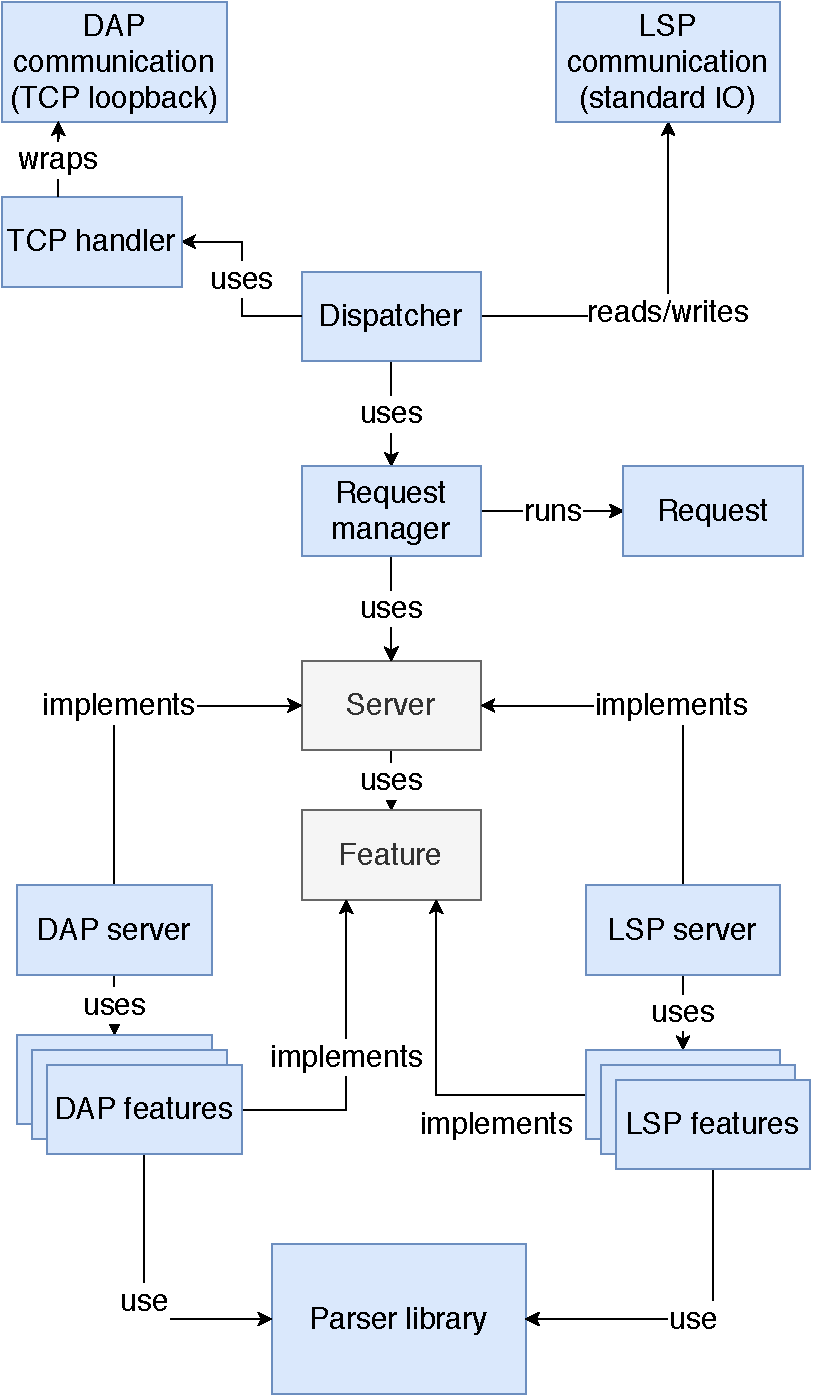
\includegraphics[width=11cm]{img/lang_server}
	\caption{Architecture of language server.}
	\label{lang_server_arch}
\end{figure}


The main purpose of the \TT{Dispatcher} is to provide abstraction for the lowest level communication, which is shared by LSP and DAP. It reads iostream to parse messages using the JSON for Modern C++ library and stores them in \TT{request manager} as requests.

A \TT{request} encapsulates one message that came from the client and basically is represented only by raw (but parsed) json.

\TT{Request manager} stores \TT{requests} in a queue and runs a worker thread that serves the requests one by one. There is only one instance of request manager running in the language server, so it serializes requests from DAP and LSP (which come asynchronously from separate sources) into one queue.

\TT{Server} is an abstract class that implements protocol behaviour that is common for both DAP and LSP --- it basically implements Remote Procedure Call. Actual handling of LSP and DAP requests is implemented in \TT{features}. Each \TT{feature} contains implementation of several protocol requests or notifications. The \TT{features} unwrap the arguments from json and call corresponding parser library methods.

Both LSP and DAP have their implementation of the abstract \TT{server} class. They both implement the initialization and finalization of protocol communication, which is a bit different for both protocols and both use features to serve protocol requests.


\section{I/O handling}
The purpose of the \TT{dispatcher} is to abstract from the complexity of working with raw strings and streams. It runs an infinite loop in which it reads messages from std::iostream and adds them to request manager as parsed json objects. At the same time, it is able to write responses in the correct format.

The language server communicates with LSP client on standard input and output, so we simply use the \TT{dispatcher} with the standard std::cin and std::cout objects to communicate with the LSP client.

The DAP communicates using TCP/IP, which is less straightforward. Before the VS Code extension starts the language server, it finds a free TCP port and passes it as an argument to the language server executable. The \TT{TCP handler} then starts listening on that port. Once the user wants to start the macro tracer, the DAP client connects to the port on localhost. The \TT{TCP handler} accepts the TCP client and creates \TT{dispatcher} and \TT{DAP server}. Once the DAP communication ends, both \TT{dispatcher} and \TT{DAP server} are destroyed and \TT{TCP handler} starts listening again for next DAP session. Thanks to the ASIO library implementation of the std::iostream interface, the dispatcher is able to completely abstract from the fact that it is communicating through TCP and not standard IO.

\section{Servers}
The servers are able to process incoming LSP and DAP requests. They get the messages in the form of already parsed jsons. Then they extract the name of requested method with its parameters from the message and call corresponding method with the parameters encoded as json.

There are two server implementations: \TT{LSP server} and \TT{DAP server}, which both inherit from abstract class \TT{server}. They implement protocol-specific processing of messages --- although the protocols are quite similar, each protocol has different initialization and finalization, different message format, etc.

The implementation of servers functionality is divided into features. Each feature implements several LSP or DAP methods by unpacking the arguments of the method and calling corresponding parser library function. At initialization, each feature adds its methods to the server's list of implemented methods. The \TT{LSP server} uses three features:
\begin{itemize}
	\item \TT{Text synchronization feature}, which handles the notifications about state of opened files in the editor
	\item \TT{Workspace folders feature}, which handles the notifications about adding and removing workspaces.
	\item \TT{Language feature}, which handles requests of HLASM code information.
\end{itemize}
The \cref{LSP_methods} shows the list of all implemented LSP methods and the class where the implementation lies.

\begin{longtable}{ll}
	\caption{The list of all implemented LSP methods and the classes where they are implemented}
	\label{LSP_methods}   \\ \toprule
	\textbf{LSP Method name} & \textbf{Component} \\ \midrule
	initialize  & LSP server     \\
	shutdown    & LSP server     \\
	exit        & LSP server    \\
	textDocument/publishDiagnostics & LSP server \\
	textDocument/didOpen  &  Text synchronization feature    \\
	textDocument/didChange  & Text synchronization feature     \\
	textDocument/didClose  &  Text synchronization feature    \\
	textDocument/semanticHighlighting & Text synchronization feature \\
	workspace/didChangeWorkspaceFolders  & Workspace folders feature     \\
	workspace/didChangeWatchedFiles  & Workspace folders feature     \\
	textDocument/definition  & Language feature     \\
	textDocument/references  & Language feature     \\
	textDocument/hover  & Language feature     \\
	textDocument/completion  & Language feature     \\ \bottomrule
\end{longtable}

The DAP server uses only one feature: Launch feature, which handles stepping through the code and retrieving information about variables and stack trace. The table \cref{DAP_methods} shows the list of all implemented DAP methods.

\begin{longtable}{ll}
	\caption{The list of all implemented DAP methods and the classes where they are implemented}
	\label{DAP_methods}   \\ \toprule
	\textbf{LSP Method name} & \textbf{Component} \\ \midrule
	initialize  & LSP server     \\
	disconnect    & LSP server     \\
	launch & Launch feature \\
	setBreakpoints  &  Launch feature    \\
	configurationDone  & Launch feature     \\
	threads  &  Launch feature    \\
	stackTrace & Launch feature \\
	scopes  & Launch feature     \\
	next  & Launch feature     \\
	stepIn  & Launch feature     \\
	variables  & Launch feature     \\
	continue  & Launch feature \\
 stopped & Launch feature \\
 exited  & Launch feature \\
 terminated & Launch feature \\\bottomrule
\end{longtable}

\section{Result respond}

According to the LSP and DAP, the server is required to send messages back to LSP/DAP client either as responds to requests(e.g. hover), notifications (e.g. textDocument/publishDiagnostics notification) or events(e.g. stopped event). Features require reference to an instance of the \TT{response provider} interface that provides methods \TT{respond} and \TT{notify} for sending messages back to LSP client. Both LSP and DAP server classes implement the \TT{response provider} to form protocol-specific correct json with the arguments.

The servers then send the json to the LSP/DAP client using the \TT{send message provider} interface. At this point, the whole json is formed, the send message provider has to add message header and serialize the json using the JSON for Modern C++ library. The only implementation of the \TT{send message provider} interface is the \TT{dispatcher}.

\section{Request Manager}

Request manager encapsulates a queue of requests with a worker thread that processes them. There may be up to two dispatcher instances in the language server: one for LSP and one for DAP. Both of them add the requests they parse into one request manager. It is necessary to process the requests one by one, because the parser library cannot process more requests at the same time.

There are three threads running in the language server:
\begin{enumerate}
	\item LSP read thread --- a thread in which Dispatcher reads messages from standard input
	\item DAP read thread --- a thread in which TCP handler listens on a localhost port to initiate DAP session. After accepting the DAP client, the dispatcher reads DAP input on this thread too.
	\item Worker thread in\TT{request manager} that processes each request using \TT{LSP server} or \TT{DAP server} and ultimately the parser library.
\end{enumerate}

The threads are synchronized in two ways: first, there is a mutex that protects adding to the request queue simultaneously by the LSP and DAP read threads. Second, there is a conditional variable to control the worker thread so it sleeps when there are no requests and wakes up when a new request has been added.

In request manager, there is a mechanism for invalidating requests that have been obsoleted by new requests. When a new request comes, all previous requests (including the one currently being processed) that are concerning the same file are invalidated. They cannot be just removed from the queue and they still have to be processed. But the parser library gets the information that the request has been obsoleted by a newer one and may behave differently.

For example, when the user starts changing a file, each character he writes comes to the language server as a textDocument/didChange notification. Normally, each such notification is processed in two parts:
\begin{itemize}
	\item Part A: the parser library changes the internal representation of the text document.
	\item Part B: the parser library starts parsing of the file to update diagnostics and highlighting. This may take some time.
\end{itemize}
When more didChange notifications come in succession, the parts A must be executed with all the notifications to keep the internal representation of the file updated. However, the user is interested only in diagnostics and semantic highlighting for the current state of the text, so we need to parse the file only once --- after the last notification.

The obsoleting of requests is done by a cancellation token. It is shared between the parser library and the request manager. When set to true, it means that the results of current request or notification are no longer needed, the parser library should stop all parsing and return as soon as possible.

\section{Example: hover request handling}

The \cref{hover_sequence} shows handling of the hover request in the language server. The hover request is sent from the LSP client to LSP server, when the user hovers over text of a file. The hover request contains the location of the mouse cursor in text, i.e. the name of the file, the number of line and column where the cursor is. The LSP client then expects a response with a string (possibly written in markdown language) to be showed in a tooltip box.

The whole process begins by the LSP instance of \TT{dispatcher} reading from the standard input. It first reads the header of message that contains information about the length of the following json. Then it reads json itself and deserializes it using the JSON for Modern C++ library. All other components of the language server work only with the parsed representation of the message. The \TT{dispatcher} adds the message to the request manager and returns to reading next message from standard input.

The request in the \TT{request manager} either waits in a queue to be processed, or if the the queue was empty then the worker thread is woken up from sleep using conditional variable. The worker then sends the json to \TT{LSP server}, which looks at the name of the method written in the message and calls the method "hover" from \TT{language feature}.

The hover method unpacks the actual arguments from json and converts any URIs to paths using the cpp-netlib URI library. Then, it calls the hover method from parser library, which returns string to be showed in tooltip next to hovering mouse. The language feature then wraps the return value back in json and calls the \TT{respond} method of its \TT{response provider} implemented by \TT{LSP server}.

The \TT{LSP server} wraps the json arguments into LSP response and uses the \TT{send message provider} implemented by \TT{Dispatcher} to send it to LSP client. The Dispatcher serializes the json, adds the header with the length of the json and writes the message to standard output. Finally, all methods return and the worker thread in request manager looks for another request. If there is none, it goes to sleep.

\begin{landscape}
	\begin{figure}
		\centering
		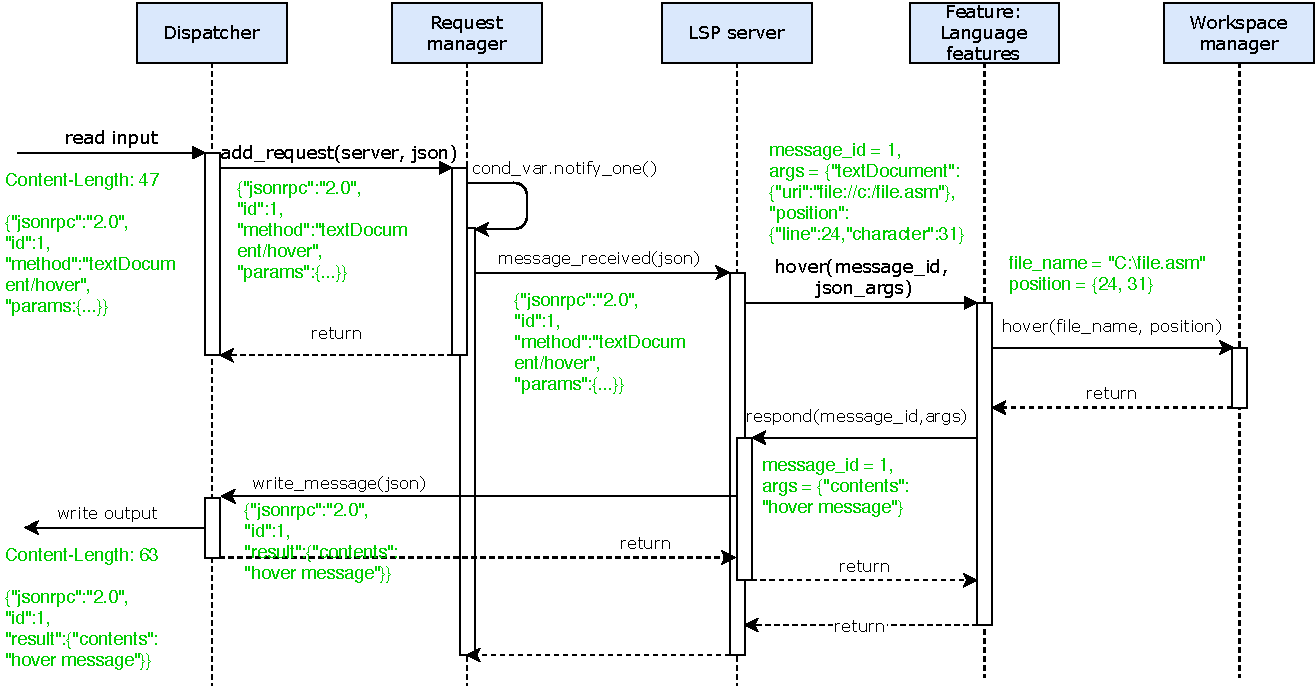
\includegraphics[width=21cm]{img/hover_sequence}
		\caption{Sequence diagram showing processing of the textDocument/hover request in the language server. The green text represents example of data passed in arguments.}
		\label{hover_sequence}
	\end{figure}
\end{landscape}


